\chapter{Анализ инструментов развертывания контейнеризированных
сред и возможности интеграции с Terraform и Scala}
\label{chapter1}

\section{Обоснование выбора Scala как языка реализации проекта}

Scala представляет собой мощный и гибкий язык программирования, который сочетает
в себе преимущества объектно-ориентированного и функционального
программирования. Вот несколько причин, почему Scala является хорошим выбором
для реализации проекта по развертыванию контейнеризированных приложений и
интеграции с Terraform:

1. \textbf{Статическая типизация}: Scala является статически типизированным
языком, что обеспечивает более высокую безопасность и надежность
программного кода. Статическая типизация позволяет выявить ошибки
на ранней стадии разработки и обеспечить более простое рефакторинг
и поддержку кода \cite{pierce-types-2012-ru}. Кроме того, Scala предоставляет
возможности для создания безопасных абстракций на уровне типов \cite{moors2008safe}.

2. \textbf{Мощные возможности абстракции}: Scala предоставляет богатый
набор инструментов для создания абстракций, таких как классы,
типажи (трейты) и высокоуровневые функции. Это позволяет разработчикам
выразить сложные операции и логику в более простой и понятной форме,
повышая читаемость и поддерживаемость кода \cite{moors2008safe}.

3. \textbf{Функциональное программирование}: Scala хорошо поддерживает
функциональное программирование, что позволяет использовать
высокоуровневые абстракции, избегать изменяемого состояния и
создавать модульный и тестируемый код. Функциональный подход
особенно полезен при работе с асинхронными операциями и обработкой ошибок.

4. \textbf{Богатая экосистема}: Scala имеет широкую экосистему библиотек
и фреймворков, которые облегчают разработку и обеспечивают доступ
к множеству полезных инструментов. Например, Cats и Cats Effect
предоставляют функциональные абстракции и типажи для упрощения
работы с эффектами и асинхронным программированием
\cite{cats-effect, cats}.

5. \textbf{Интеграция с Java и JVM}: Scala полностью совместима с Java
и может взаимодействовать с существующими Java-библиотеками и
инфраструктурой. Это дает возможность использовать богатую экосистему
Java и переиспользовать существующий код и инструменты.

6. \textbf{Поддержка функционального комбинаторного программирования}:
Scala имеет поддержку для функциональной комбинаторной логики, которая
может быть полезна для моделирования и анализа систем
\cite{wolfengagen-combinatory-2008, wolfengagen-methods-2008}.
Это может быть полезно при разработке алгебраического описания для
представления объектов Terraform и других частей проекта.

В целом, Scala предлагает разработчикам мощные инструменты и гибкость,
которые могут быть полезны при реализации проекта по развертыванию
контейнеризированных приложений и интеграции с Terraform. Она позволяет
создавать высококачественный, типобезопасный и модульный код, что важно
для разработки сложных систем.

\section{Обзор системы Terraform и методов обеспечения интеграции с ней}

Terraform - это инструмент открытого исходного кода, разработанный HashiCorp,
для безопасного и эффективного управления облачной инфраструктурой как
кодом (IaC) \cite{jourdan2017infrastructure}. Terraform позволяет определить и
предоставить полную инфраструктуру данных, серверов, сетей и приложений в
различных облачных сервисах, таких как AWS, Google Cloud, Azure и других, а
также в локальных средах, таких как VMware и OpenStack \cite{howard2022terraform}.

Terraform использует декларативный подход, что означает, что вы описываете
желаемое состояние инфраструктуры, а Terraform заботится о том, как достичь
этого состояния. Это упрощает управление сложными системами и уменьшает
вероятность ошибок.

Terraform предоставляет множество провайдеров, которые позволяют
взаимодействовать с различными облачными сервисами и другими сервисами.
Каждый провайдер предоставляет набор ресурсов, которые можно управлять
с помощью Terraform. Например, провайдер AWS предоставляет ресурсы,
такие как $aws\_instance$ и $aws\_vpc$, которые можно использовать для
управления экземплярами EC2 и VPC в AWS \cite{howard2022terraform}.

Terraform поддерживает модули, что позволяет группировать и повторно
использовать ресурсы. Модули могут быть использованы для создания
абстракций высокого уровня, что упрощает управление сложными системами.

Terraform также поддерживает состояние, что позволяет отслеживать
текущее состояние инфраструктуры и применять изменения инкрементно.
Это уменьшает вероятность ошибок и упрощает управление сложными системами.

Для интеграции Terraform с другими системами, такими как Scala или
Kubernetes, можно использовать провайдеры Terraform, модули и другие
функции Terraform. Например, можно использовать провайдер Kubernetes
для управления ресурсами Kubernetes с помощью Terraform, или можно
использовать Scala для типизации всех структур
Terraform \cite{shapkin-automation-2022}, на примере того,
как это описано в данной статье, для последующей
генерации файлов конфигурации Terraform.

Важно отметить, что Terraform предоставляет множество возможностей
для автоматизации и управления облачной инфраструктурой, но он также
требует знания и понимания облачных сервисов и концепций IaC.
Поэтому важно провести тщательное исследование и планирование перед
использованием Terraform в проекте.

В заключение, Terraform представляет собой мощный инструмент для
управления облачной инфраструктурой как кодом. Он предлагает гибкость
и контроль, которые требуются для управления сложными системами,
и предоставляет множество возможностей для интеграции с другими
системами и инструментами. Однако, как и любой мощный инструмент,
он требует знания и понимания для эффективного использования.

\section{Анализ системы Kubernetes и её особенностей типизации}

Kubernetes - это открытая система для автоматизации развертывания,
масштабирования и управления контейнеризированными приложениями.
Она была разработана Google и сейчас поддерживается Cloud Native Computing
Foundation \cite{bernstein-containers-2014}.

Одной из ключевых особенностей Kubernetes является её система типов
ресурсов. В Kubernetes каждый объект, такой как под, служба или том,
имеет определенный тип. Эти типы определяют свойства и действия, которые
могут быть применены к объектам. Например, поды представляют собой
наименьшую и простейшую единицу в модели развертывания Kubernetes,
которая создает и управляет контейнерами \cite{sayfan2017mastering}.

Типизация в Kubernetes обеспечивает гибкость и контроль при управлении
ресурсами. Она позволяет пользователям определять и управлять ресурсами
в соответствии с их потребностями и требованиями. Типизация также
обеспечивает безопасность и изоляцию, позволяя пользователям контролировать
доступ к ресурсам и изолировать их от других ресурсов \cite{bijon2014formal}.

Однако, типизация в Kubernetes также может быть сложной и трудной для
понимания, особенно для новых пользователей. Она требует глубокого
понимания концепций Kubernetes и может вызвать сложности при интеграции
с другими системами и инструментами.

Для упрощения работы с типизацией в Kubernetes можно использовать
различные инструменты и библиотеки. Например, можно использовать
библиотеку клиентского API \newline Kubernetes для работы с объектами Kubernetes
в программном коде. Также можно использовать инструменты командной строки,
такие как kubectl, для управления ресурсами Kubernetes \cite{kubectl}.

Важной частью системы Kubernetes является планировщик (scheduler),
который отвечает за распределение подов по узлам кластера. Планировщик
принимает решения на основе различных факторов, таких как доступность
ресурсов, требования к аффинности и анти-аффинности, ограничения на уровне
узла и т.д. \cite{carrion2022kubernetes}.

Также стоит отметить, что Kubernetes сам по себе потребляет определенное
количество ресурсов для своей работы. Это включает в себя ресурсы,
необходимые для работы компонентов управления Kubernetes, таких как
API-сервер, планировщик и контроллер-менеджер, а также ресурсы, необходимые
для работы служб, таких как DNS и сетевые плагины \cite{turin2023predicting}.
Понимание этих затрат на ресурсы важно для эффективного планирования и
управления кластерами Kubernetes.

В заключение, Kubernetes предлагает мощную и гибкую систему типов для
управления контейнеризированными приложениями. Однако, как и любая мощная
система, она требует знания и понимания для эффективного использования.

\section{Исследование возможностей интеграции системы Kubernetes с \newline
Terraform}
Kubernetes и Terraform могут быть интегрированы для автоматизации процесса
развертывания и управления контейнеризированными приложениями.
Это может быть особенно полезно в больших и сложных средах, где ручное
управление может быть трудоемким и подвержено ошибкам.
Такая интеграция в подобных средах позволила бы автоматически изменять
структуру серверов в зависимости от нагрузки на кластер Kubernetes. 
Это позволило бы увеличивать количество серверов во время пиковых нагрузок
и снижать в моменты простоя (например ночью).

Одним из способов интеграции Kubernetes и Terraform является использование
провайдера Kubernetes в Terraform. Этот провайдер позволяет Terraform
взаимодействовать с кластером Kubernetes, позволяя пользователям описывать
и управлять ресурсами Kubernetes в коде Terraform. Это позволяет
пользователям использовать преимущества Terraform, такие как планирование
изменений, управление версиями и модульность, при работе с Kubernetes.
Однако данный способ никак не позволяет управлять серверами
Kubernetes, что делает его непригодным для оптимизации серверной
инфраструктуры Kubernetes \cite{davis2021bootstrapping}.

Другим способом интеграции может быть использование API Kubernetes
для сопоставления серверов, на которых настроен Kubernetes, с серверами,
указанными в декларации Terraform. Это может быть полезно для обеспечения
согласованности между реальной инфраструктурой и ее описанием в коде
Terraform.

Однако, интеграция Kubernetes и Terraform может представлять собой
некоторые сложности. Например, может быть сложно обеспечить согласованность
между состоянием инфраструктуры, описанной в коде Terraform,
и реальным состоянием кластера Kubernetes. Кроме того, может
потребоваться дополнительная настройка и конфигурация для обеспечения
безопасности и изоляции при использовании этих инструментов вместе.

В заключение, интеграция Kubernetes и Terraform предлагает множество
преимуществ для автоматизации и управления контейнеризированными
приложениями. Однако, как и любая интеграция, она требует тщательного
планирования и управления для обеспечения эффективности и безопасности.

\section{Анализ возможностей использования формальных методов при
моделировании ресурсов IaaS}
Инфраструктура как услуга (IaaS) представляет собой модель облачных
вычислений, которая предоставляет виртуальные вычислительные ресурсы
через Интернет. IaaS является одной из трех основных категорий облачных
вычислений, наряду с Платформой как услуга (PaaS) и Программным обеспечением
как сервис (SaaS) \cite{iaas2017}.

Формальные методы представляют собой подход к проектированию и анализу
систем, который использует строгие математические модели для описания
и проверки свойств системы. Формальные методы могут быть использованы
для моделирования различных аспектов IaaS, включая управление ресурсами,
изоляцию и безопасность 
\cite{bijon2014formal, amato2018improving, de2012formal}.

Управление ресурсами в IaaS включает в себя распределение и
оркестрацию вычислительных ресурсов, таких как процессорное время,
память и сетевые ресурсы. Формальные методы могут быть использованы
для создания математических моделей этих процессов, что позволяет
проанализировать их свойства и гарантировать их корректность
\cite{de2012formal, turin2023predicting}.

Изоляция в IaaS относится к способности системы изолировать ресурсы и
приложения друг от друга, чтобы предотвратить взаимное влияние и
обеспечить безопасность. Формальные методы могут быть использованы
для моделирования и анализа механизмов изоляции, что позволяет
гарантировать их эффективность и безопасность \cite{bijon2014formal}.

Безопасность в IaaS включает в себя защиту данных и приложений от
несанкционированного доступа и атак. Формальные методы могут быть
использованы для моделирования и анализа механизмов безопасности,
что позволяет гарантировать их корректность и надежность
\cite{amato2018improving}.

В заключение, формальные методы предлагают мощный инструментарий для
моделирования и анализа IaaS. Они могут помочь обеспечить корректность,
эффективность и безопасность систем IaaS, что является критически важным
для облачных сервисов. Они позволяют разработчикам и архитекторам
систематически анализировать и проверять свойства системы на ранних
стадиях проектирования, что может значительно снизить риски и стоимость
исправления ошибок в более поздних стадиях жизненного цикла системы.

\section{Сравнение k3s, Kubernetes, Minikube}

Kubernetes, k3s и Minikube представляют собой различные инструменты
для работы с контейнеризированными приложениями, каждый из которых
имеет свои особенности и преимущества.

Kubernetes является стандартом де-факто в области оркестрации
контейнеров и предлагает широкий спектр функциональности для управления,
масштабирования и обеспечения безопасности контейнеризированных
приложений. Однако его сложность и требовательность к ресурсам могут
быть препятствием для некоторых сценариев использования, особенно в
средах с ограниченными ресурсами или для разработчиков, которые только
начинают работать с контейнерами.

K3s, разработанный Rancher Labs, представляет собой легковесную версию
Kubernetes, которая упрощает процесс развертывания и управления
контейнерами. K3s удаляет некоторые функции Kubernetes, которые
не требуются в большинстве развертываний, такие как облачные
контроллеры провайдеров и альфа-функции, что позволяет уменьшить
требования к ресурсам и упростить установку и настройку. В статье
Böhm и Wirtz (2021) было показано, что k3s обеспечивает
сопоставимую производительность с Kubernetes при значительно
меньших требованиях к ресурсам \cite{bohm2021profiling}.

Minikube представляет собой инструмент, который позволяет локально
развертывать однонодовой кластер Kubernetes на персональном компьютере
разработчика. Это делает его идеальным инструментом для разработки и 
тестирования приложений Kubernetes в локальной среде перед их
развертыванием в производственной среде. Minikube поддерживает все
основные функции Kubernetes и предлагает ряд дополнительных функций,
таких как поддержка различных драйверов виртуализации и интеграция с
инструментами CI/CD.

В целом, выбор между Kubernetes, k3s и Minikube будет зависеть от
конкретных требований и сценариев использования. Kubernetes предлагает
наиболее полный набор функций и подходит для больших и сложных
развертываний. K3s является хорошим выбором для сред с
ограниченными ресурсами или когда требуется упрощенная установка и
настройка. Согласно исследованию Böhm и Wirtz (2021), k3s обеспечивает
сопоставимую производительность с Kubernetes, но при значительно меньших
требованиях к ресурсам \cite{bohm2021profiling}.

Minikube, с другой стороны, идеально подходит для локальной
разработки и тестирования. Он позволяет развертывать кластер из нескольких
виртуальных нод Kubernetes на персональном компьютере разработчика,
поддерживает все основные функции Kubernetes и предлагает ряд
дополнительных функций, таких как поддержка различных драйверов
виртуализации и интеграция с инструментами CI/CD.

Таким образом, при выборе между Kubernetes, k3s и
Minikube следует учитывать специфику задач, требования
к ресурсам и уровень сложности установки и настройки.


\section{Архитектура Kubernetes}

Kubernetes — это портативная, расширяемая платформа с открытым исходным кодом
для управления контейнеризированными рабочими нагрузками и сервисами. Она
обеспечивает как декларативную конфигурацию, так и автоматизацию. В основе
архитектуры Kubernetes лежат \textit{поды} (Pods)  — наименьшие развертываемые единицы,
которые можно создать и управлять \cite{nocentino2021kubernetes}.

\subsection*{Компоненты управления}
Центральные компоненты управления Kubernetes, известные как \textit{плоскость управления}
(control plane), включают:

\begin{itemize}
   \item \textbf{Kube-API сервер} (\textit{kube-apiserver}): предоставляет API
Kubernetes, через который выполняется взаимодействие с кластером.
   \item \textbf{Схема данных etcd}: надежное хранилище для всех данных
кластера Kubernetes.
   \item \textbf{Контроллеры} (\textit{Controller Manager}): управляют
основными циклами Kubernetes, такими как репликация подов, отслеживание
состояний узлов (нод) и многое другое.
   \item \textbf{Планировщик} (\textit{Scheduler}): отвечает за размещение
подов на узлах в соответствии с доступными ресурсами и требованиями подов.
\end{itemize}

\subsection*{Рабочие узлы и компоненты}
Рабочие узлы включают в себя следующие компоненты:

\begin{itemize}
   \item \textbf{Kubelet}: агент, работающий на каждом узле, управляет подами и
их контейнерами.
   \item \textbf{Kube-Proxy}: сетевой прокси, обеспечивающий сетевую связь
внутри кластера Kubernetes.
   \item \textbf{Контейнерная среда выполнения} (\textit{Container Runtime}):
программное обеспечение для запуска контейнеров.
\end{itemize}

\subsection*{Объекты Kubernetes}
Kubernetes использует различные абстракции для представления состояния системы:

\begin{itemize}
   \item \textbf{Поды} (\textit{Pods}): группа одного или нескольких
контейнеров, совместно использующих хранилище и сетевые ресурсы.
   \item \textbf{Сервисы} (\textit{Services}): абстракция, обеспечивающая
постоянный доступ к группе подов.
   \item \textbf{Развертывания} (\textit{Deployments}): управляют созданием и
обновлением подов и их реплик.
   \item \textbf{Тома} (\textit{Volumes}): предоставляют хранилище, доступное
для подов.
\end{itemize}

\begin{figure}[h]
   \centering
   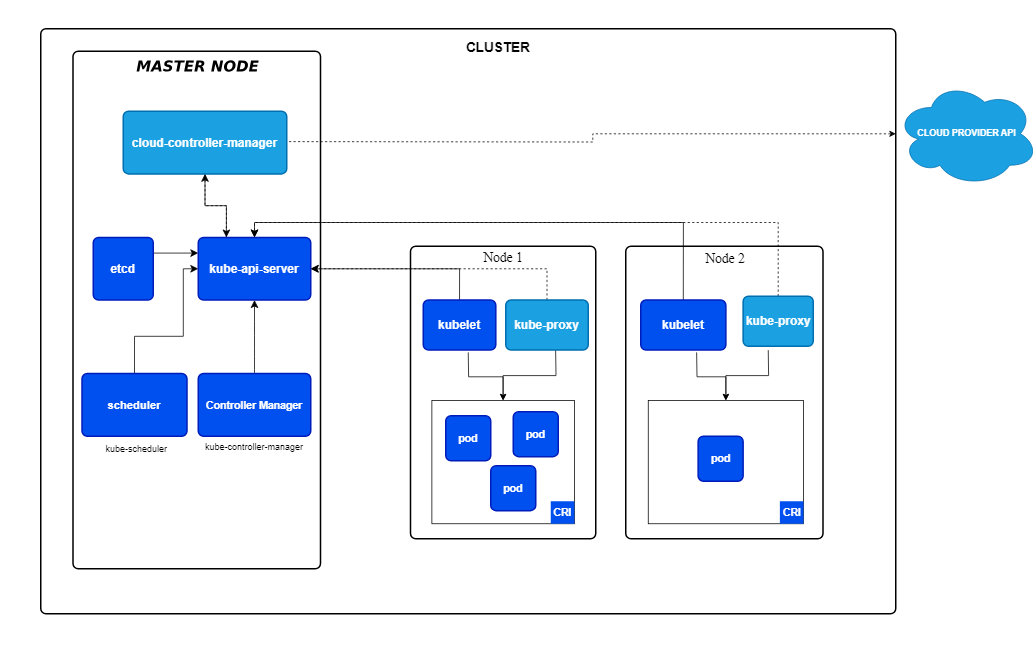
\includegraphics[scale=0.4]{img/8.png}
   \caption{Архитектура Kubernetes}
   \label{fig:ccg}
 \end{figure}

Эта многоуровневая архитектура обеспечивает масштабируемость, устойчивость и
управляемость распределенных систем, что является ключевым фактором в
обеспечении эффективной работы современных микросервисных приложений.

\subsection*{Планировщик Kubernetes (Kubernetes Scheduler)}

Планировщик Kubernetes (\textit{Scheduler}) играет ключевую роль в распределении
подов (\textit{Pods}) по узлам (\textit{Nodes}) кластера. Основная задача
планировщика — выбор подходящего узла для каждого нового пода на основе доступных
ресурсов и требований пода \cite{luksa2017kubernetes}.
Работа планировщика включает следующие этапы:

\begin{enumerate}
   \item \textbf{Сбор информации (Information Gathering)}: Сбор информации о
требованиях пода, таких как ресурсы CPU и памяти, аффинность узлов и
допустимые (толерантности) узлы.
   \item \textbf{Фильтрация узлов (Node Filtering)}: Проверка узлов на соответствие
требованиям пода.
   \item \textbf{Ранжирование узлов (Node Scoring)}: Ранжирование подходящих узлов
на основе различных критериев, таких как общее количество ресурсов, близость к
другим важным подам или специфические политики распределения.
   \item \textbf{Выбор узла (Node Selection)}: Выбор узла с наивысшим рангом
для размещения пода.
\end{enumerate}

\subsection*{Отказоустойчивость подов (Pod Fault Tolerance)}

Отказоустойчивость в Kubernetes достигается через механизмы восстановления и
репликации подов:

\begin{itemize}
   \item \textbf{Репликация (Replication)}: Контроллеры, такие как
\textit{ReplicaSet}, гарантируют, что указанное количество копий пода всегда
запущено. Если под терпит сбой, контроллер автоматически создает новый под для
замены.
   \item \textbf{Самовосстанавливающиеся процессы (Self-Healing Processes)}: Если узел
становится недоступным, планировщик Kubernetes перераспределяет поды этого узла
на другие доступные узлы.
   \item \textbf{Стратегии развертывания (Deployment Strategies)}: Механизмы,
такие как \textit{Rolling Update} в объектах \textit{Deployment}, обеспечивают
постоянное обновление подов без простоя.
\end{itemize}

\subsection*{Жизненный цикл подов (Pod Lifecycle)}

Жизненный цикл подов в Kubernetes включает следующие этапы:

\begin{enumerate}
   \item \textbf{Создание пода (Pod Creation)}: Пользователь или контроллер
создает объект пода, и API сервер записывает его в etcd.
   \item \textbf{Планирование (Scheduling)}: Планировщик Kubernetes выбирает
подходящий узел для пода.
   \item \textbf{Запуск (Launching)}: Kubelet на назначенном узле запускает
контейнеры внутри пода, используя указанную контейнерную среду выполнения.
   \item \textbf{Работа (Running)}: Под остается в рабочем состоянии, пока он
выполняет свои функции. Контроллеры наблюдают за его состоянием и
восстанавливают его при сбоях.
   \item \textbf{Удаление (Termination)}: После остановки пода (через API
сервер) Kubelet удаляет под с узла.
\end{enumerate}

Эти механизмы обеспечивают эффективное распределение и управление ресурсами, а
также повышают устойчивость и надежность работы кластера Kubernetes.

\section*{Обзор виртуальных машин в Yandex Cloud и Rustack}

В современных облачных вычислениях виртуальные машины (VM) играют ключевую роль,
обеспечивая гибкость и масштабируемость ресурсов. Yandex Cloud и Rustack
предлагают передовые решения в этой области, применяя различные подходы и
технологии.

\textbf{Yandex Cloud} \cite{yandexcloud} использует виртуализацию на уровне
гипервизора для
развертывания VM. Это обеспечивает высокую изоляцию и безопасность каждой VM,
позволяя пользователям настраивать свои экземпляры в соответствии с
индивидуальными требованиями. Yandex Cloud предлагает широкий спектр настроек
VM, включая различные конфигурации процессора, памяти и хранилища. Сетевая
инфраструктура Yandex Cloud обеспечивает высокопроизводительное подключение и
безопасность, включая виртуальные частные сети (VPN), балансировщики нагрузки и
защиту от DDoS-атак.

\textbf{Rustack} \cite{rustack}, с другой стороны, фокусируется на предоставлении
более гибких
и настраиваемых решений в области облачных вычислений. Платформа позволяет
пользователям создавать VM с высокой степенью контроля над конфигурацией и
управлением ресурсами. Rustack поддерживает интеграцию с различными облачными и
физическими сетями, предоставляя эффективные средства для настройки сетевой
инфраструктуры, включая продвинутые опции маршрутизации и брандмауэра.

Оба провайдера поддерживают автоматизацию и оркестрацию с помощью API и
инструментов управления инфраструктурой, таких как Terraform и Ansible, что
позволяет эффективно масштабировать и управлять ресурсами. Интеграция с
современными инструментами разработки и CI/CD обеспечивает плавную интеграцию VM
в процессы разработки и развертывания.

В заключение, Yandex Cloud и Rustack предлагают разнообразные возможности для
работы с виртуальными машинами, каждый со своими уникальными преимуществами, что
делает их подходящими для различных сценариев использования в области облачных
вычислений.

\section{Выводы}

В данной главе проанализированы инструменты развертывания контейнеризированных
сред и их интеграция с Terraform и Scala. Выделены ключевые преимущества Scala,
включая статическую типизацию, мощные возможности абстракции и поддержку функционального 
программирования. Terraform оценен как мощный инструмент для управления облачной 
инфраструктурой, предлагающий гибкость, контроль и возможности интеграции. 
Kubernetes рассмотрен с точки зрения типизации ресурсов и управления
контейнеризированными приложениями, подчеркивая его мощную и гибкую систему типов. 
Исследованы возможности интеграции Kubernetes и Terraform, подчеркивая потенциал 
автоматизации и вызовы согласованности. Подчеркнута значимость формальных методов 
для моделирования ресурсов IaaS, обеспечивая корректность, эффективность и безопасность. 
Проведено сравнение k3s, Kubernetes и Minikube, выделяя их применение в различных 
сценариях в зависимости от требований и ресурсов. Представлен обзор архитектуры 
Kubernetes, включая компоненты управления, рабочие узлы, объекты, планировщик и 
жизненный цикл подов. Наконец, Yandex Cloud и Rustack представлены как гибкие
решения для работы с виртуальными машинами в области облачных вычислений, 
предлагая различные подходы и технологии.

\section{Постановка задачи курсового проекта}

Целью данного курсового проекта является апробация системы автомасштабирования
кластера Kubernetes на платформах РУСТЭК и/или Яндекс Облако. В рамках проекта
предполагается выполнение следующих ключевых задач:

\begin{enumerate}
 \item \textbf{Изучение Механизмов Автомасштабирования Kubernetes:} Детальный
анализ существующих механизмов автомасштабирования в Kubernetes, включая
изучение алгоритмов \cite{senjab2023survey}, политик и стратегий масштабирования 
\cite{tran2022survey, qu2018auto, millnert2020holoscale}.
 
 \item \textbf{Выбор и Настройка Платформы:} Определение критериев для выбора
между платформами РУСТЭК и Яндекс Облако для развертывания кластера Kubernetes и
настройка соответствующей инфраструктуры.
 
 \item \textbf{Реализация и Интеграция Системы Автомасштабирования:} Разработка
системы автомасштабирования с учетом требований к эффективности распределения ресурсов 
\cite{zhong2020cost}, её интеграция с кластером Kubernetes на выбранной
платформе, настройка метрик и пороговых значений для масштабирования.
 
 \item \textbf{Экспериментальное Тестирование:} Проведение экспериментов для
оценки эффективности системы автомасштабирования, включая моделирование
различных сценариев нагрузки.
 
 \item \textbf{Анализ Результатов и Оптимизация:} Анализ данных
экспериментального тестирования и внесение корректировок для улучшения
эффективности и надежности системы.
 
 \item \textbf{Оценка Применимости и Эффективности:} Оценка применимости и
эффективности реализованной системы автомасштабирования в контексте реальных
рабочих нагрузок на платформах РУСТЭК и/или Яндекс Облако.
\end{enumerate}

В результате выполнения проекта ожидается получение эффективной системы
автомасштабирования для кластеров Kubernetes, способной адаптироваться к
изменениям в рабочей нагрузке и обеспечивающей оптимальное использование
ресурсов на выбранных облачных платформах.